%----------------------------------------------------------------------------------------
%	PACKAGES AND OTHER DOCUMENT CONFIGURATIONS
%----------------------------------------------------------------------------------------

\documentclass[
	11pt, % Set the default font size, options include: 8pt, 9pt, 10pt, 11pt, 12pt, 14pt, 17pt, 20pt
	%t, % Uncomment to vertically align all slide content to the top of the slide, rather than the default centered
	aspectratio=169, % Uncomment to set the aspect ratio to a 16:9 ratio which matches the aspect ratio of 1080p and 4K screens and projectors
]{beamer}

\graphicspath{{figures/}{./}} % Specifies where to look for included images (trailing slash required)

\usepackage{booktabs} % Allows the use of \toprule, \midrule and \bottomrule for better rules in tables
\usepackage{caption}
\usepackage{tikz}
\usepackage{amsmath}
\usepackage{amssymb}
\usepackage{placeins}
\usepackage{mathtools}
\usepackage{hyperref}

\hypersetup{%
  colorlinks=false,% hyperlinks will be coloured
  linkcolor=brown,% hyperlink text will be green
  linkbordercolor=blue,% hyperlink border will be red
}

%----------------------------------------------------------------------------------------
%	SELECT LAYOUT THEME
%----------------------------------------------------------------------------------------

% Beamer comes with a number of default layout themes which change the colors and layouts of slides. Below is a list of all themes available, uncomment each in turn to see what they look like.

%\usetheme{default}
%\usetheme{AnnArbor}
%\usetheme{Antibes}
%\usetheme{Bergen}
%\usetheme{Berkeley}
%\usetheme{Berlin}
%\usetheme{Boadilla}
%\usetheme{CambridgeUS}
%\usetheme{Copenhagen}
%\usetheme{Darmstadt}
%\usetheme{Dresden}
%\usetheme{Frankfurt}
%\usetheme{Goettingen}
%\usetheme{Hannover}
%\usetheme{Ilmenau}
%\usetheme{JuanLesPins}
%\usetheme{Luebeck}
\usetheme{Madrid}
%\usetheme{Malmoe}
%\usetheme{Marburg}
%\usetheme{Montpellier}
%\usetheme{PaloAlto}
%\usetheme{Pittsburgh}
%\usetheme{Rochester}
%\usetheme{Singapore}
%\usetheme{Szeged}
%\usetheme{Warsaw}

%----------------------------------------------------------------------------------------
%	SELECT COLOR THEME
%----------------------------------------------------------------------------------------

% Beamer comes with a number of color themes that can be applied to any layout theme to change its colors. Uncomment each of these in turn to see how they change the colors of your selected layout theme.

%\usecolortheme{albatross}
%\usecolortheme{beaver}
%\usecolortheme{beetle}
%\usecolortheme{crane}
%\usecolortheme{dolphin}
%\usecolortheme{dove}
%\usecolortheme{fly}
% \usecolortheme{lily}
% \usecolortheme{monarca}
% \usecolortheme{seagull}
%\usecolortheme{seahorse}
%\usecolortheme{spruce}
% \usecolortheme{whale}
%\usecolortheme{wolverine}

%----------------------------------------------------------------------------------------
%	SELECT FONT THEME & FONTS
%----------------------------------------------------------------------------------------

% Beamer comes with several font themes to easily change the fonts used in various parts of the presentation. Review the comments beside each one to decide if you would like to use it. Note that additional options can be specified for several of these font themes, consult the beamer documentation for more information.

\usefonttheme{default} % Typeset using the default sans serif font
%\usefonttheme{serif} % Typeset using the default serif font (make sure a sans font isn't being set as the default font if you use this option!)
%\usefonttheme{structurebold} % Typeset important structure text (titles, headlines, footlines, sidebar, etc) in bold
%\usefonttheme{structureitalicserif} % Typeset important structure text (titles, headlines, footlines, sidebar, etc) in italic serif
%\usefonttheme{structuresmallcapsserif} % Typeset important structure text (titles, headlines, footlines, sidebar, etc) in small caps serif

%------------------------------------------------

%\usepackage{mathptmx} % Use the Times font for serif text

%\usepackage{helvet} % Use the Helvetica font for sans serif text
%\usepackage[default]{FiraSans} % Use the Fira Sans font for sans serif text
%\usepackage[default]{lato} % Use the Lato font for sans serif text

%----------------------------------------------------------------------------------------
%	SELECT INNER THEME
%----------------------------------------------------------------------------------------

% Inner themes change the styling of internal slide elements, for example: bullet points, blocks, bibliography entries, title pages, theorems, etc. Uncomment each theme in turn to see what changes it makes to your presentation.

%\useinnertheme{default}
\useinnertheme{circles}
%\useinnertheme{rectangles}
%\useinnertheme{rounded}
%\useinnertheme{inmargin}

%----------------------------------------------------------------------------------------
%	SELECT OUTER THEME
%----------------------------------------------------------------------------------------

% Outer themes change the overall layout of slides, such as: header and footer lines, sidebars and slide titles. Uncomment each theme in turn to see what changes it makes to your presentation.

%\useoutertheme{default}
%\useoutertheme{infolines}
%\useoutertheme{miniframes}
%\useoutertheme{smoothbars}
%\useoutertheme{sidebar}
%\useoutertheme{split}
%\useoutertheme{shadow}
%\useoutertheme{tree}
%\useoutertheme{smoothtree}

%\setbeamertemplate{footline} % Uncomment this line to remove the footer line in all slides
%\setbeamertemplate{footline}[page number] % Uncomment this line to replace the footer line in all slides with a simple slide count

%\setbeamertemplate{navigation symbols}{} % Uncomment this line to remove the navigation symbols from the bottom of all slides

%----------------------------------------------------------------------------------------
%	PRESENTATION INFORMATION
%----------------------------------------------------------------------------------------

\title[New Optimizer I]{New Optimizer I} % The short title in the optional parameter appears at the bottom of every slide, the full title in the main parameter is only on the title page

\subtitle{} % Presentation subtitle, remove this command if a subtitle isn't required

\author[]{Alexander Ludwig} % Presenter name(s), the optional parameter can contain a shortened version to appear on the bottom of every slide, while the main parameter will appear on the title slide


\date[\today]{Deep Learning Research Kitchen (ML-4501 / 3 ECTS) \\ \today} % Presentation date or conference/meeting name, the optional parameter can contain a shortened version to appear on the bottom of every slide, while the required parameter value is output to the title slide

%----------------------------------------------------------------------------------------

\AtBeginSection[]{
  \begin{frame}
  \vfill
  \centering
  \begin{beamercolorbox}[sep=8pt,center,shadow=true,rounded=true]{title}
    \usebeamerfont{title}\insertsectionhead\par%
  \end{beamercolorbox}
  \vfill
  \end{frame}
}

\begin{document}

%----------------------------------------------------------------------------------------
%	TITLE SLIDE
%----------------------------------------------------------------------------------------

\begin{frame}
	\titlepage % Output the title slide, automatically created using the text entered in the PRESENTATION INFORMATION block above
\end{frame}

%----------------------------------------------------------------------------------------
%	TABLE OF CONTENTS SLIDE
%----------------------------------------------------------------------------------------

% The table of contents outputs the sections and subsections that appear in your presentation, specified with the standard \section and \subsection commands. You may either display all sections and subsections on one slide with \tableofcontents, or display each section at a time on subsequent slides with \tableofcontents[pausesections]. The latter is useful if you want to step through each section and mention what you will discuss.

\begin{frame}
	\frametitle{Structure} % Slide title, remove this command for no title
	
	\tableofcontents % Output the table of contents (all sections on one slide)
	%\tableofcontents[pausesections] % Output the table of contents (break sections up across separate slides)
\end{frame}

%----------------------------------------------------------------------------------------
%	PRESENTATION BODY SLIDES
%----------------------------------------------------------------------------------------

\section{New and popular optimizers} % Sections are added in order to organize your presentation into discrete blocks, all sections and subsections are automatically output to the table of contents as an overview of the talk but NOT output in the presentation as separate slides

%------------------------------------------------

\subsection{AdamW}

\begin{frame}
	\frametitle{AdamW: decoupling weight decay from your adaptive optimizer}
	\framesubtitle{More state of the art research from Freiburg}
	 \begin{columns}[c] % The "c" option specifies centered vertical alignment while the "t" option is used for top vertical alignment
		\begin{column}{0.55\textwidth} % Left column width
			\begin{itemize}
				\item Given a loss $L(\theta) = \hdots + \lambda \vert \vert \theta \vert \vert^2 $ ($L_2 regularization$)
				\item only for vanilla SGD this is equivalent to \textbf{weight decay} \\
				 $\theta_{t+1} = \theta_t - \eta( \dots + \lambda \theta_t) $\\
				 \vspace{1em}
				 $\Longrightarrow$ first update $\theta_{t+1} = -\eta \lambda \theta_t$ then \textit{continue}
				 \item AdamW is one of the best practice optimizers (at least firmly ingrained in \href{https://github.com/karpathy/nanoGPT}{NanoGPT})

			\end{itemize}
		\end{column}
		\begin{column}{0.35\textwidth} % Right column width
        	\begin{figure}
        	    \centering
                
\includegraphics[width=8cm]{figures/adamw.png}
        	    \caption*{}
        	\end{figure}
		\end{column}
	\end{columns}
\end{frame}

\subsection{Recap 2nd Order methods}
\begin{frame}
	\frametitle{But why should we stick to first order methods?}
	\framesubtitle{Reminder: Antionio's Lecture and Newton's Method}
		"With $H= L \cdot I_{dxd}$ the theory is perfect" \\
		"the optimal $\eta$, yielding the maximum decrease is $\eta = 1/L$ "\\
		\vspace{1em}
		\textbf{{Hessian Matrix}}, $\theta \in \mathbb{R}^d$
\[
H = \begin{bmatrix}
\frac{\partial^2 L}{\partial \theta_1^2} & \frac{\partial^2 L}{\partial \theta_1 \partial \theta_2} & \cdots & \frac{\partial^2 L}{\partial \theta_1 \partial \theta_n} \\
\frac{\partial^2 L}{\partial \theta_2 \partial \theta_1} & \frac{\partial^2 L}{\partial \theta_2^2} & \cdots & \frac{\partial^2 L}{\partial \theta_2 \partial \theta_n} \\
\vdots & \vdots & \ddots & \vdots \\
\frac{\partial^2 L}{\partial \theta_n \partial \theta_1} & \frac{\partial^2 L}{\partial \theta_n \partial \theta_2} & \cdots & \frac{\partial^2 L}{\partial \theta_n^2}
\end{bmatrix} \in \textcolor{red}{\mathbb{R}^{d\times d}}
\]

		\textbf{Newton's Method}: $\theta_{t+1} = \theta_t - H^{\textcolor{red}{-1}} g$\\
		"quadratic convergence for convex problems"

\end{frame}

\begin{frame}
	\frametitle{Gauss-Newton-Bartlett Estimator }
	\framesubtitle{making the Hessian diagonal and linearize a deep neural network}
	Reminder: the multivariate Chain Rule $L: L(f_1(x), f_2(x), \dots, f_c(x))$:\[
\frac{\partial L}{\partial x_i}(f(x)) = \sum_{j=1}^c \frac{\partial L}{\partial f_j} \frac{\partial f_j}{\partial x_i} = \nabla_f L  J_x
\]
				 \begin{align*}
					H_{ij} &= \frac{\partial^2 L}{\partial \theta_i \partial \theta_j} =\frac{\partial}{\partial \theta_i }\left( \sum_j \frac{\partial L}{\partial f_j} \frac{\partial f_j}{\partial \theta_i}  \right) 
				 =\left( \sum_j \frac{\partial}{\partial \theta_i } \left(\frac{\partial L}{\partial f_j}\right) \frac{\partial f_j}{\partial \theta_i} +    \frac{\partial L}{\partial f_j} \frac{\partial}{\partial \theta_i }\left( \frac{\partial f_j}{\partial \theta_i}\right) \right) \\
				 &=\textcolor{magenta}{\left( \sum_j \sum_k \frac{\partial^2 L }{\partial f_j \partial f_k }  \frac{\partial f_j}{\partial \theta_i} \frac{\partial f_k}{\partial \theta_j}\right)}+ \sum_j \left(  \frac{\partial L}{\partial f_j} \underbrace{\frac{\partial}{\partial \theta_i }\left( \frac{\partial f_j}{\partial \theta_i}\right)}_{=0 \text{ for linear}f} \right)  = \textcolor{magenta}{J_\theta^T \underset{\in \mathbb{R}^{c\times c}}{H_f} J_\theta} +  smol
				 \end{align*}
\end{frame}
 
\begin{frame}
	\frametitle{GNB 2\footnote{\href{https://youtu.be/416NjW3QfwA?feature=shared}{Here} is great Lecture about Second Order Optimizer from the Numerics of ML lecture by Lukas Tatzel}}
	Since $L=H(p_{\text{data}}, p_{\text{model}}) = E_{x\sim p_{data}}[-\log(p_{model}(x))]$ one can rewrite  $H_f = E_{\hat{y} \sim p_{model}}[\frac{\partial^2 L }{\partial^2 f }] =E_{\hat{y} \sim p_{model}}[\frac{\partial L }{\partial f }\frac{\partial L }{\partial f }^T] $ ($H_f$ does no independent on $\hat{y}$)\\
	$\rightarrow G = E[J_\theta \frac{\partial L }{\partial f }\frac{\partial L }{\partial f }^T J_\theta^T] = E_{\hat{y} \sim p_{model}}[\nabla_\theta L \odot \nabla_\theta L] $
	\begin{itemize}
		\item splitting up second derivatives in expectation is called Bartlett's second identity 
		\item sample $\hat{y} \sim p_{model}$ and calculate gradient w.r.t. $L$
	\end{itemize}

	
\end{frame}
%------------------------------------------------

\subsection{Sophia}
\begin{frame}{Sophia}
	\framesubtitle{\textbf{S}econd-\textbf{o}rder Clip\textbf{p}ed Stoc\textbf{h}astic Opt\textbf{i}miz\textbf{a}tion}
	 \begin{columns}[c] % The "c" option specifies centered vertical alignment while the "t" option is used for top vertical alignment
		\begin{column}{0.45\textwidth} % Left column width
			\begin{itemize}
				\item accounts for curvature information during optimization
				\item clips gradient at 1
				\item "The authors suspect the GNB estimator has a smaller variance than the Hutchinson’s
				estimator, [...]."
				\item public implementation is only with GNB available
				\item Hessian diagonal is approximated every $k$ steps
			\end{itemize}
		\end{column}
		\begin{column}{0.55\textwidth} % Right column width
        	\begin{figure}
        	    \centering
                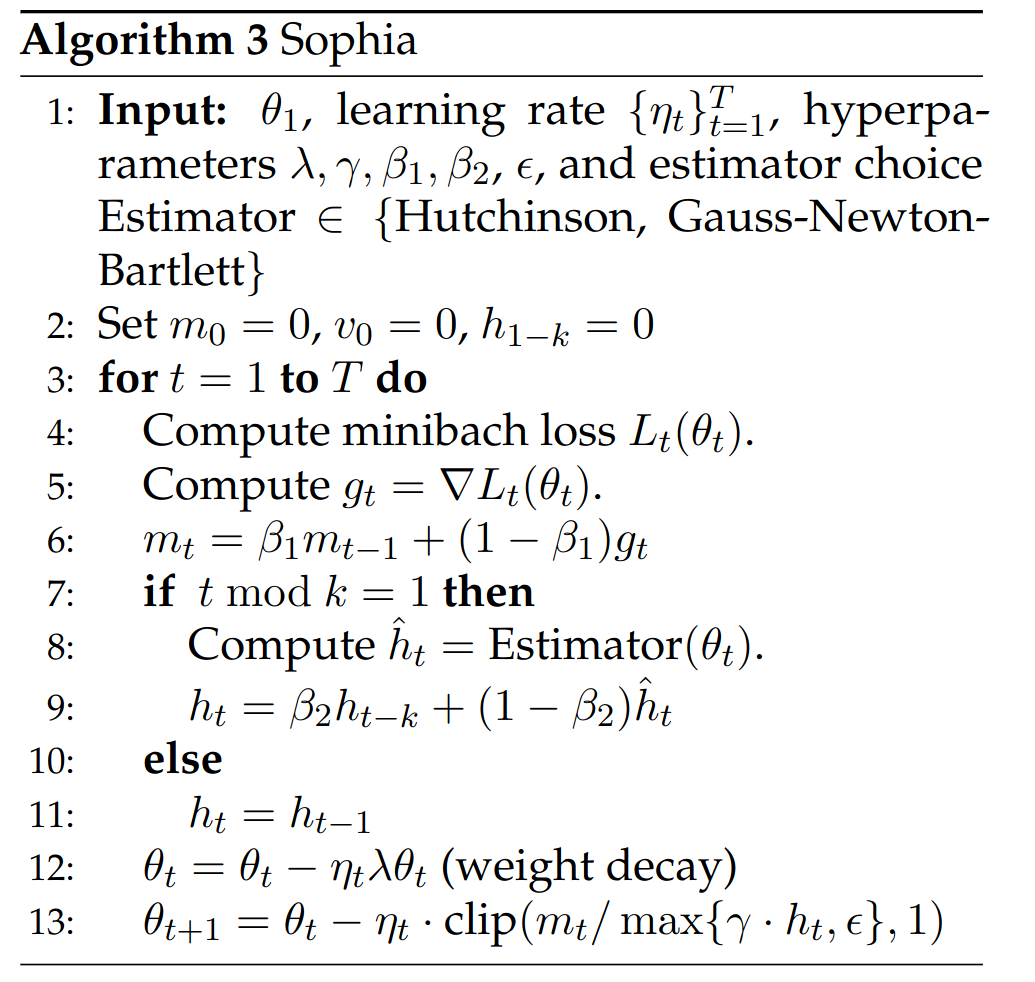
\includegraphics[width=6.5cm]{figures/sophia_algo.png}
        	    \caption*{Claude Shannon}
        	\end{figure}
		\end{column}
	\end{columns}
\end{frame}

\begin{frame}{Defining 2x faster }
\begin{columns}[c] % The "c" option specifies centered vertical alignment while the "t" option is used for top vertical alignment
		\begin{column}{0.45\textwidth} % Left column width
			\begin{figure}
				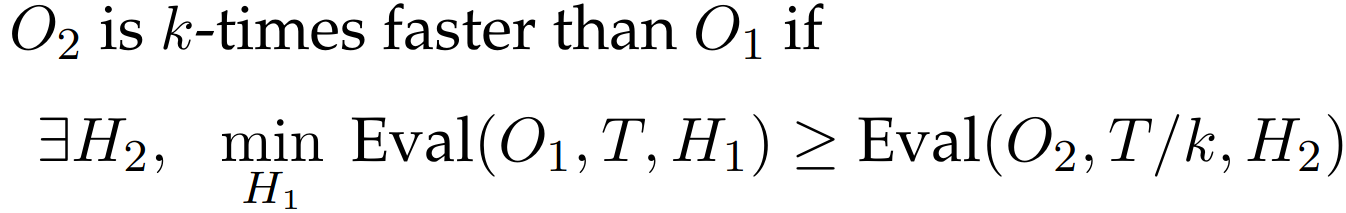
\includegraphics[width=7cm]{figures/2xfaster.png}
			\end{figure}
		\end{column}
		\begin{column}{0.55\textwidth} % Right column width
        	\begin{figure}
        	    \centering
                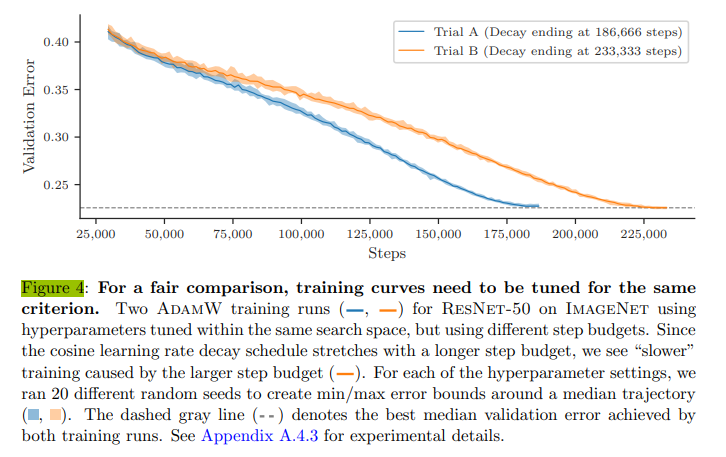
\includegraphics[width=7.5cm]{figures/figure4_dahl_et_al.PNG}
        	\end{figure}
		\end{column}
	\end{columns}
\end{frame}


%------------------------------------------------

\subsection{Lion}

\begin{frame}{Lion: EvoLved Sign Momentum, an attempt to gödelize optimizers }
	\framesubtitle{Why not breed your dream optimizer via evolution }
	\vspace{-1em}
\begin{columns}[c] % The "c" option specifies centered vertical alignment while the "t" option is used for top vertical alignment
		\begin{column}{0.45\textwidth} % Left column width
			\begin{itemize}
					\item regularized evolution searches through the symbolic representations					
					\item inputs are weights, lr and gradient; output can be weights update + extra stuff
					\item performance is measured on ViT on 10\% of Imagenet (20 mins TPU) and very tiny on LM1B
					\item limited vocabulary and constants are modified/ newly sampled a la $2^a$ for $a\sim \mathcal{N}(0,1)$
					\item prune search space by checking for functional equivalence and redundant statements 
					\item tons of compute at google helps
			\end{itemize}
		\end{column}
		\begin{column}{0.55\textwidth} % Right column width
        	\begin{figure}
        	    \centering
                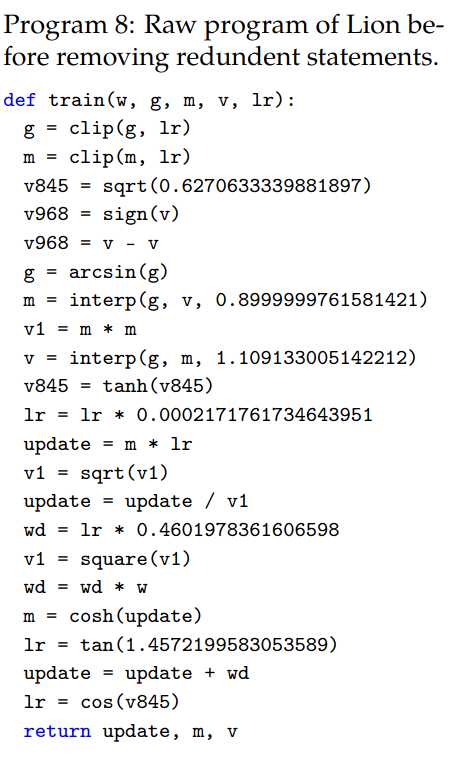
\includegraphics[width=4.4cm]{figures/raw_lion.png}
        	\end{figure}
		\end{column}
	\end{columns}
\end{frame}



\begin{frame}{Lion 2}
	\framesubtitle{Optimizing NNs is already searching over TMs, where will this lead to when we now start searching optimizers?}
	 \begin{columns}[c] % The "c" option specifies centered vertical alignment while the "t" option is used for top vertical alignment
		\begin{column}{0.45\textwidth} % Left column width
				\begin{itemize}
					\item decoupled weight decay is added manually (gray lines)
					\item \texttt{interp(a,b,$\lambda$) = $(1-\lambda) a + \lambda b$ } 
					\item uniform update direction across \textbf{all} dimensions of $\theta$
					\item authors argue that sign operation adds noise to gradient update and regularizes
					\item smaller memory footprint than AdamW (only momentum stored)
					\item almost the same as signSGD (moment variant)
				\end{itemize}
		\end{column}
		\begin{column}{0.55\textwidth} % Right column width
        	\begin{figure}
        	    \centering
                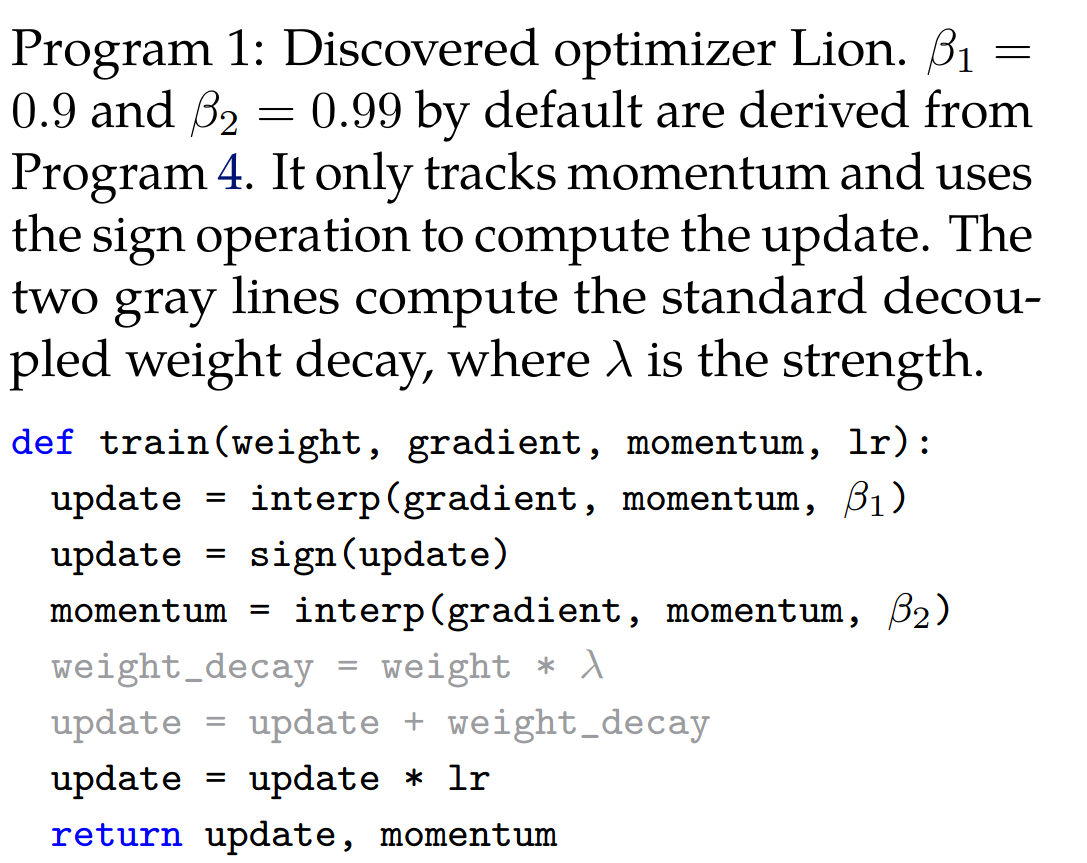
\includegraphics[width=6.5cm]{figures/signMomentum.png}
        	    \caption*{Cleaned up optimizer }
        	\end{figure}
		\end{column}
	\end{columns}
\end{frame}

\subsection{Experiments}

\begin{frame}{Experiments}
		\begin{figure}[ht]
        \centering
		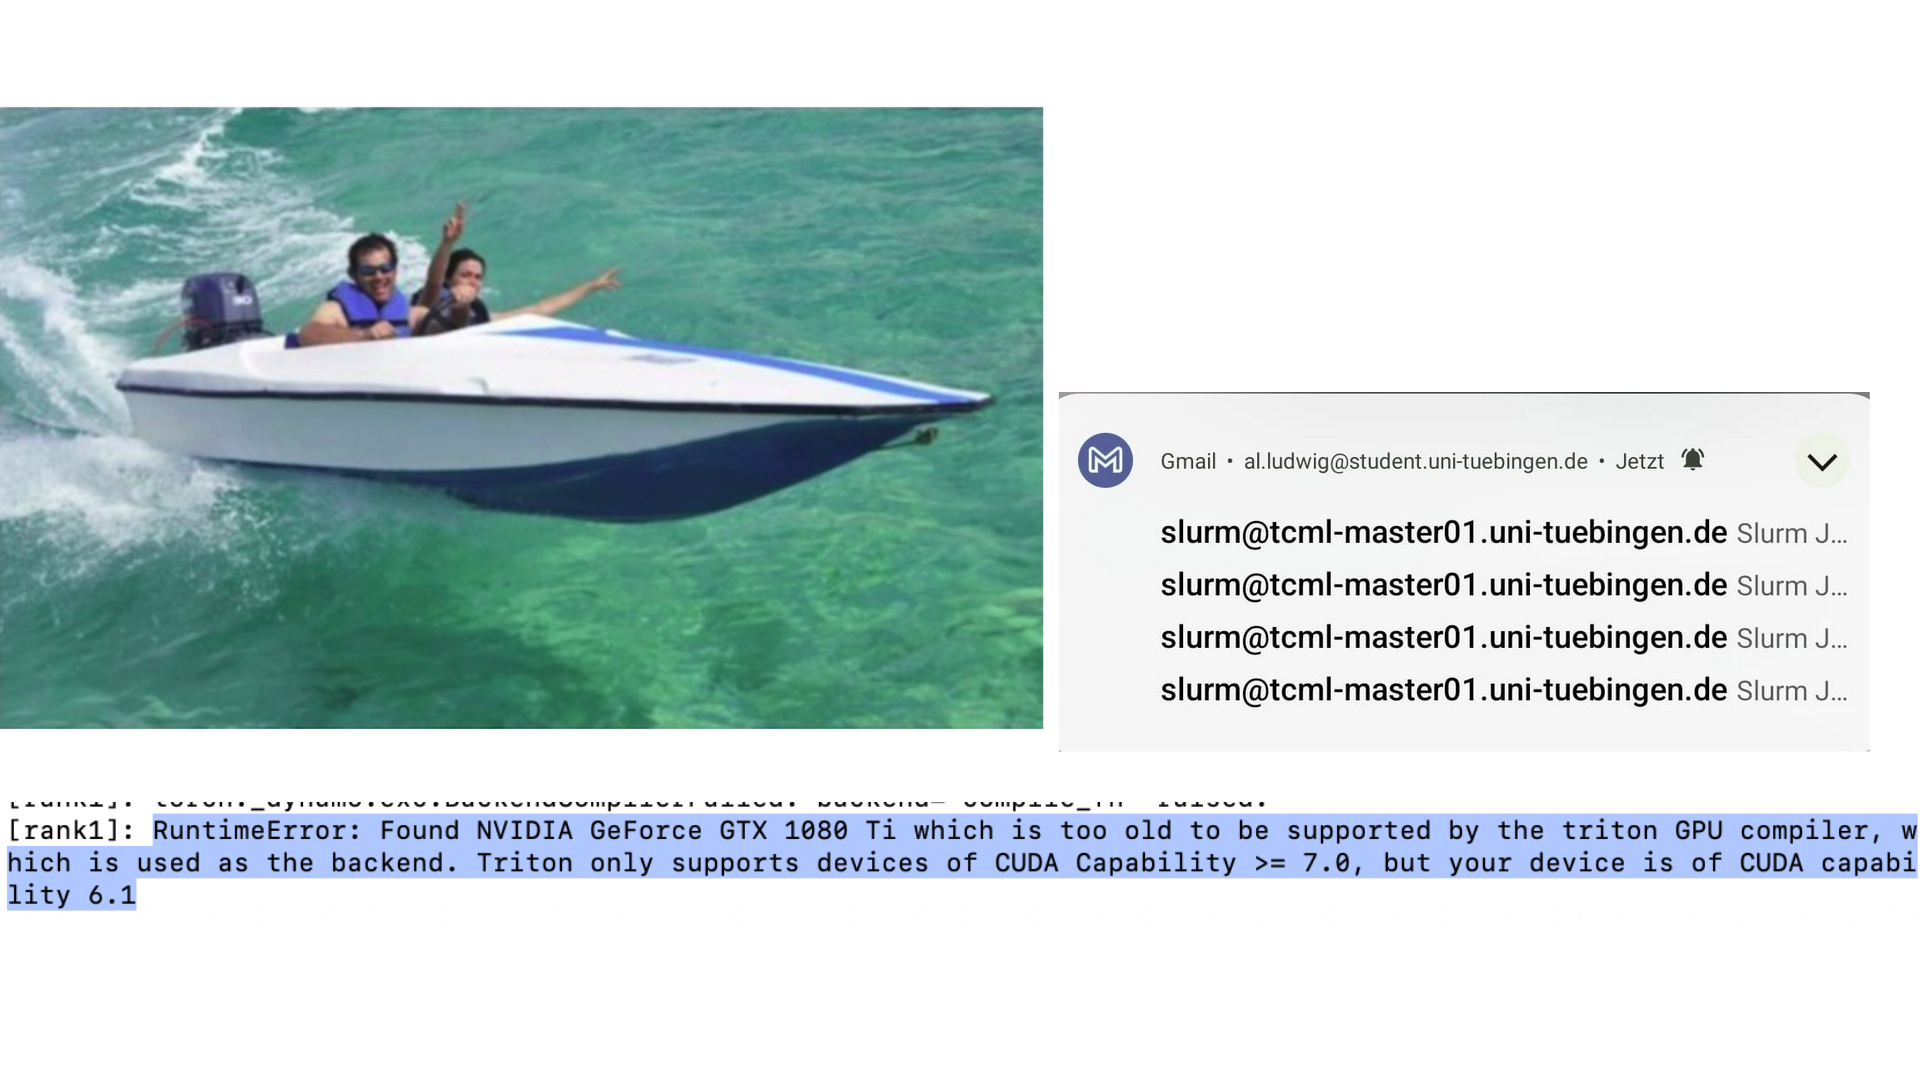
\includegraphics[width=14cm]{figures/NanoGPTFUN.png}
        \caption{Graphical representation of a Latent Variable Model. $\mathbf{Z}$ is called the latent variable and  $X_i$ the target message.}
        \label{fig:LVM}
    \end{figure}
\end{frame}

\begin{frame}
		\begin{figure}[ht]
        \centering
		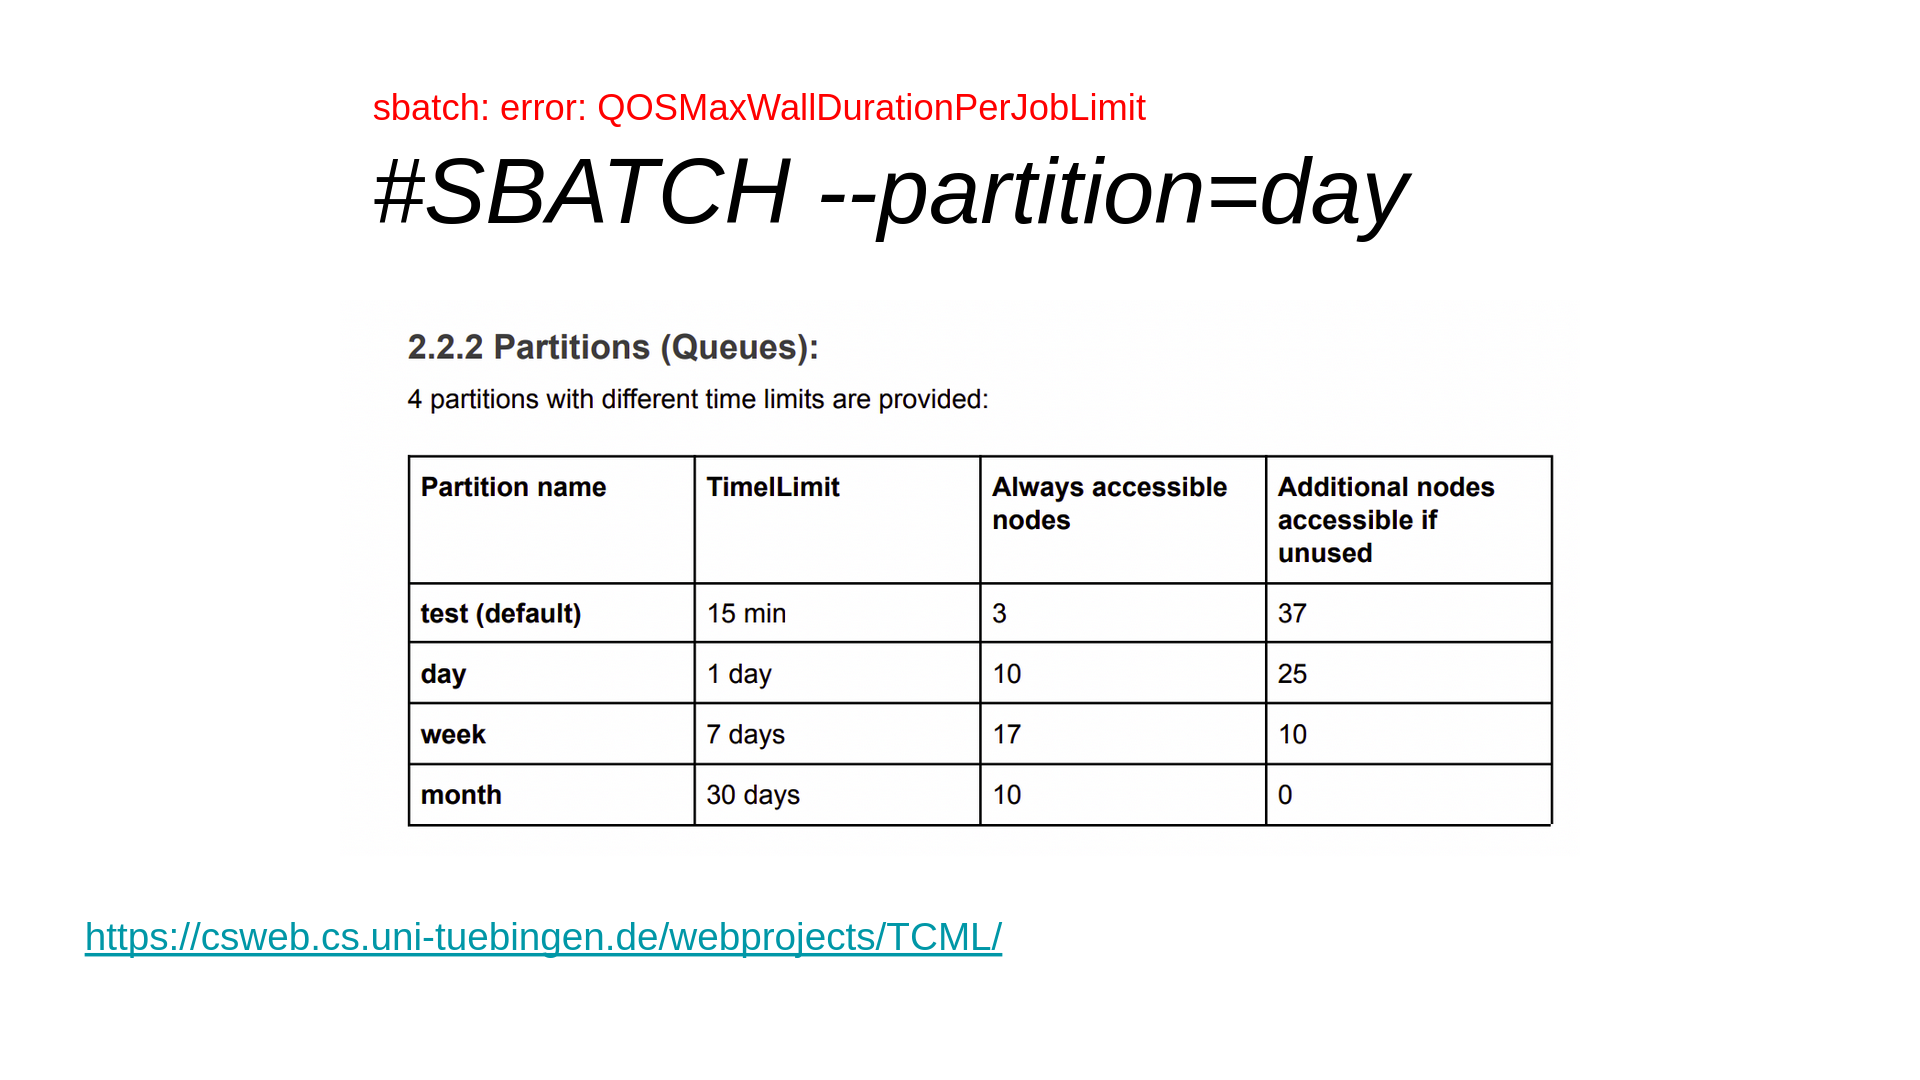
\includegraphics[width=14cm]{figures/cluster_advice.png}
    \end{figure}
\end{frame}

 \begin{frame}
	\frametitle{Setup}
	\begin{itemize}
		\item All Experiments are run on the tcml cluster on a single computer node with 4x GeForce GTX 1080 Ti and Intel XEON CPU E5-2650 v4 (24 cores)
		\item fork of Sophia repository which itself is a fork of \href{https://github.com/karpathy/nanoGPT/tree/master}{NanoGPT repository} by Andrej Karpathy
		\item 10K update steps during training on data from \href{https://openwebtext2.readthedocs.io/en/latest/}{OpenWebText 2}
		\item cross entropy loss 
		\item Cosine learning rate schedule with 200 steps warmup
		\item \textit{tiny} transformer (30M parameters, 6 Layers, 6 attention heads, 384 embedding dimension, context length of 1024 tokens)
		\item \textit{gradient accumulation} was used to simulate a higher batch size (120 most of the time)
	\end{itemize}
\end{frame}

%------------------------------------------------

 \begin{frame}
	\frametitle{Hyperparameters }
	\begin{itemize}
		\item Sophia paper reports \textit{optimal} hyperparameters for tiny model on 50K (40K more) steps for different optimizers
		\item increase maximum learning rate until divergence
	\end{itemize}
	\begin{figure}
		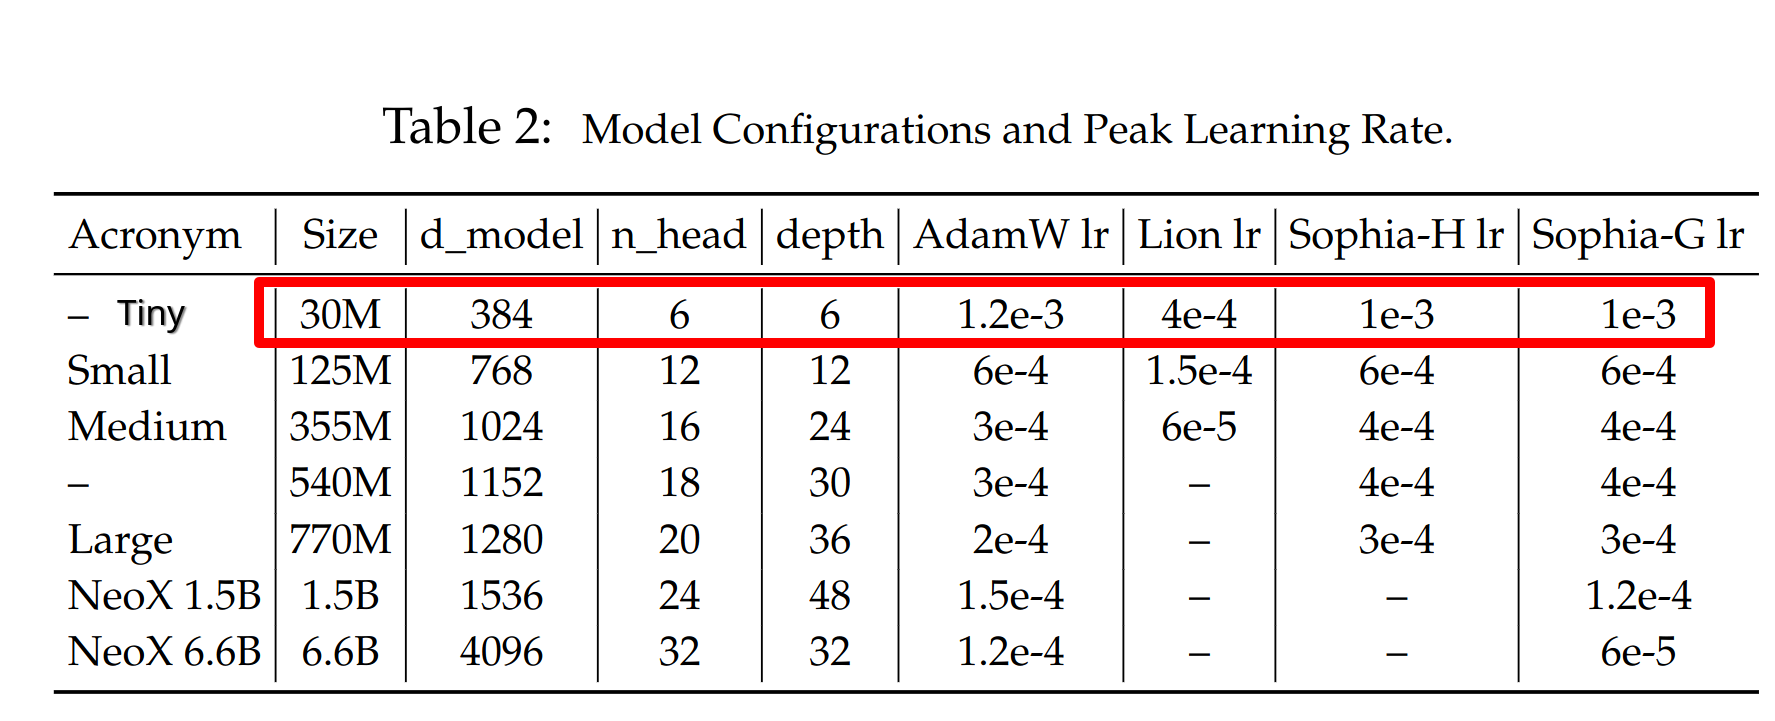
\includegraphics[width=10cm]{figures/hyperparams_from_sophia.png}
		\caption*{adapted from Appendix B from Liu et.al 2024}
	\end{figure}
\end{frame}

%------------------------------------------------
 \begin{frame}
	\frametitle{Sophia vs AdamW: 2x faster in \#steps or time?}
	\begin{figure}
		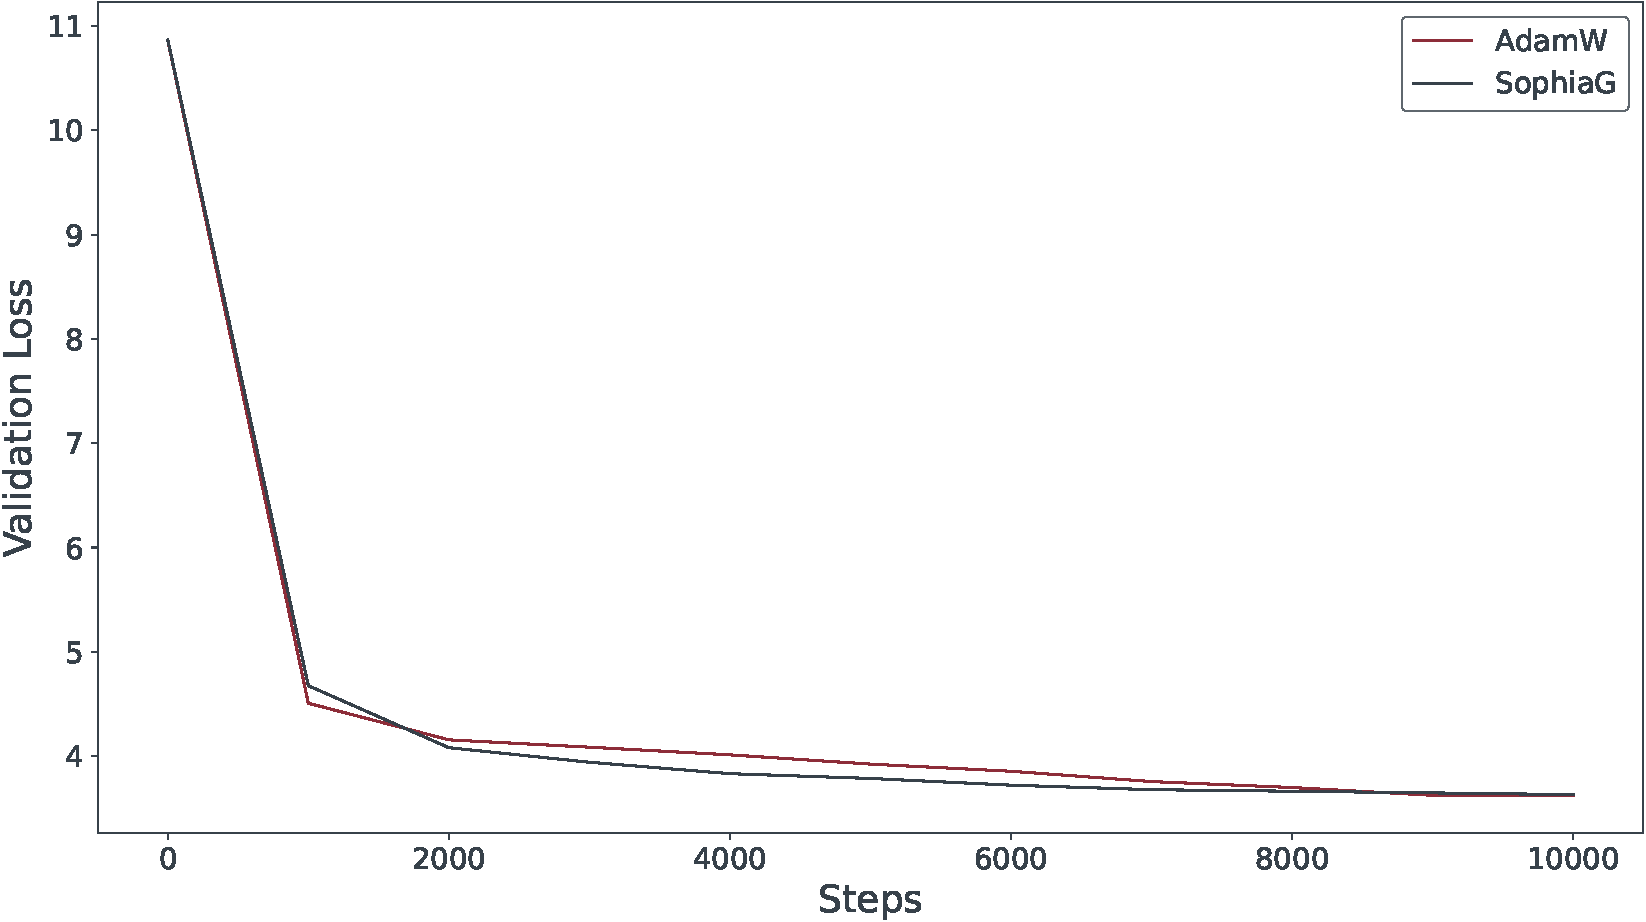
\includegraphics[width=12cm]{../results/steps_adam_sophia.pdf}
		\caption{lowest validation losses: AdamW: 3.621 bits, SophiaG: 3.669 bits}
	\end{figure}
\end{frame}


\begin{frame}[plain] % The optional argument 'plain' hides the headline and footline

	\begin{figure}
		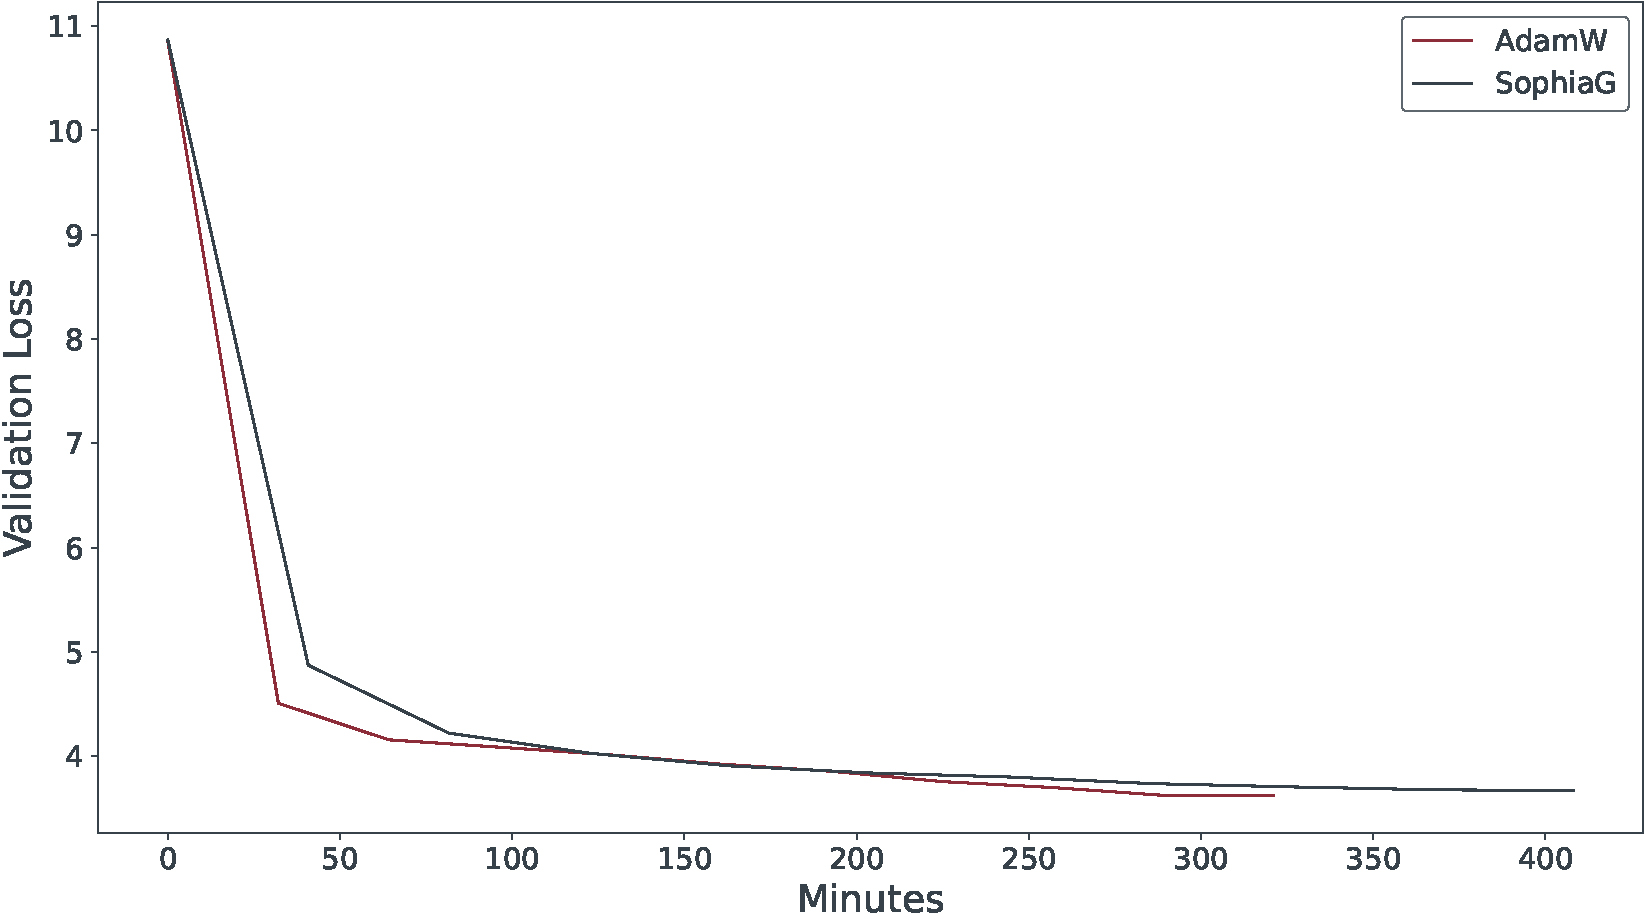
\includegraphics[width=12cm]{../results/time_adam_sophia.pdf}
		\caption*{Both optimizer performed 10K steps but different wallclock times: AdamW 5h 21m, SophiaG: 6h 48m}
	\end{figure}
\end{frame}
%------------------------------------------------
\begin{frame}{} % The optional argument 'plain' hides the headline and footline

	\begin{figure}
		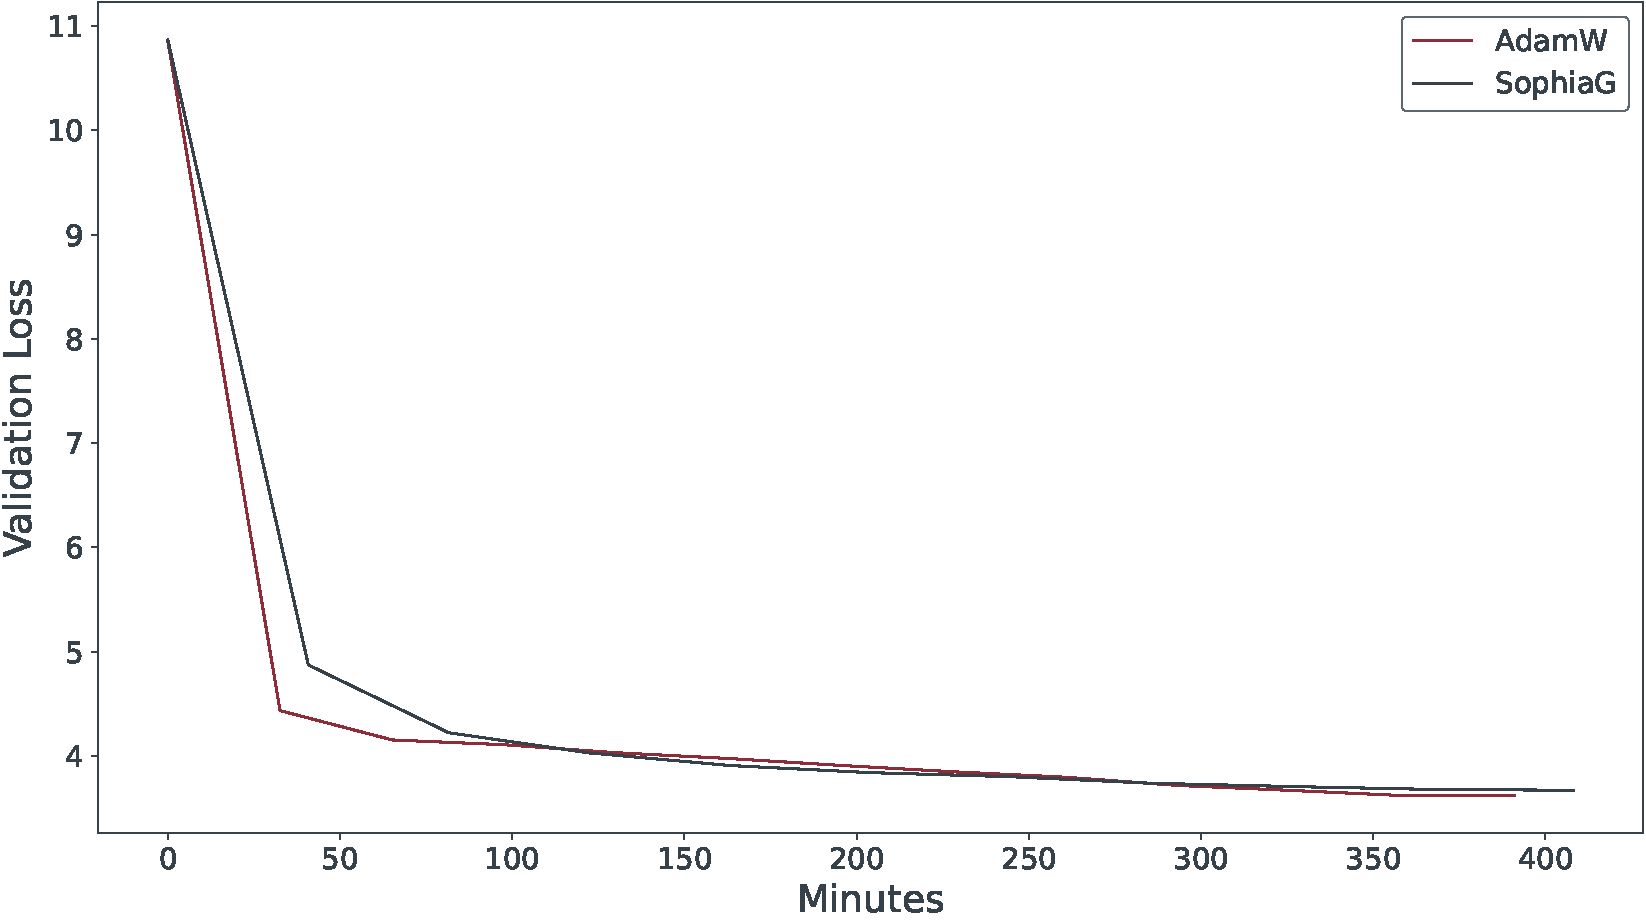
\includegraphics[width=12cm]{../results/time_adam_long_sophia.pdf}
		\caption*{Both optimizer run for approx. the same time: AdamW 6h 31m, SophiaG: 6h 48m}
	\end{figure}
\end{frame}

 \begin{frame}
 \frametitle{Caveats}
 \begin{itemize}
	\item Since they don't report loss values for tiny (30M) model on 10K steps, this is \textbf{not} a "falsification" of their claims
	\item SophiaG run on 5k steps does also not achieve lower validation loss
	\item $\dots$
 \end{itemize}
\end{frame}


\begin{frame}{Releasing the Lion}
 \begin{figure}
	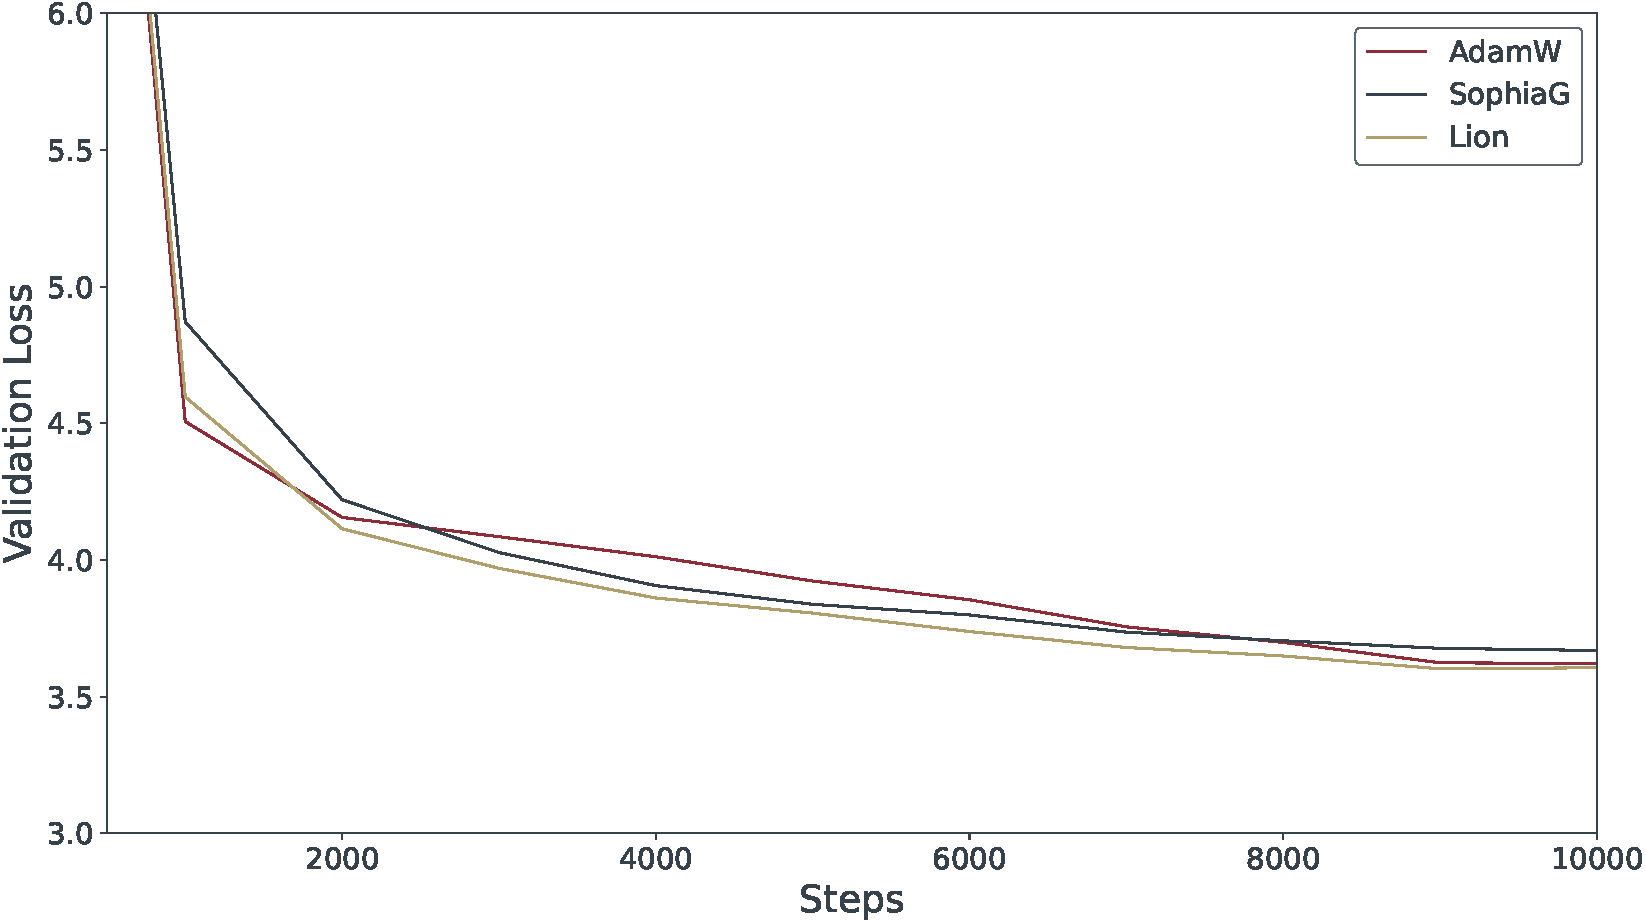
\includegraphics[width=12cm]{../results/lion_adam_sophia.pdf}
	\caption*{Validation Losses: Lion 3.606 bits, AdamW 3.621 bits, SophiaG 3.669 bits}
 \end{figure}
\end{frame}

%------------------------------------------------


\section{Conclusion and Discussion}
\begin{frame}[plain] % The optional argument 'plain' hides the headline and footline
	\begin{center}
		{\Huge Thank you for your attention! }
		
		\bigskip\bigskip % Vertical whitespace
		
		{\LARGE Any questions, comments or Feedback? 
\includegraphics[width=1cm]{figures/vae.png}}
		
\includegraphics[width=5cm]{qr_to_wandb.png}
	\end{center}
\end{frame}

\begin{frame}[plain] % The optional argument 'plain' hides the headline and footline
	\begin{center}
		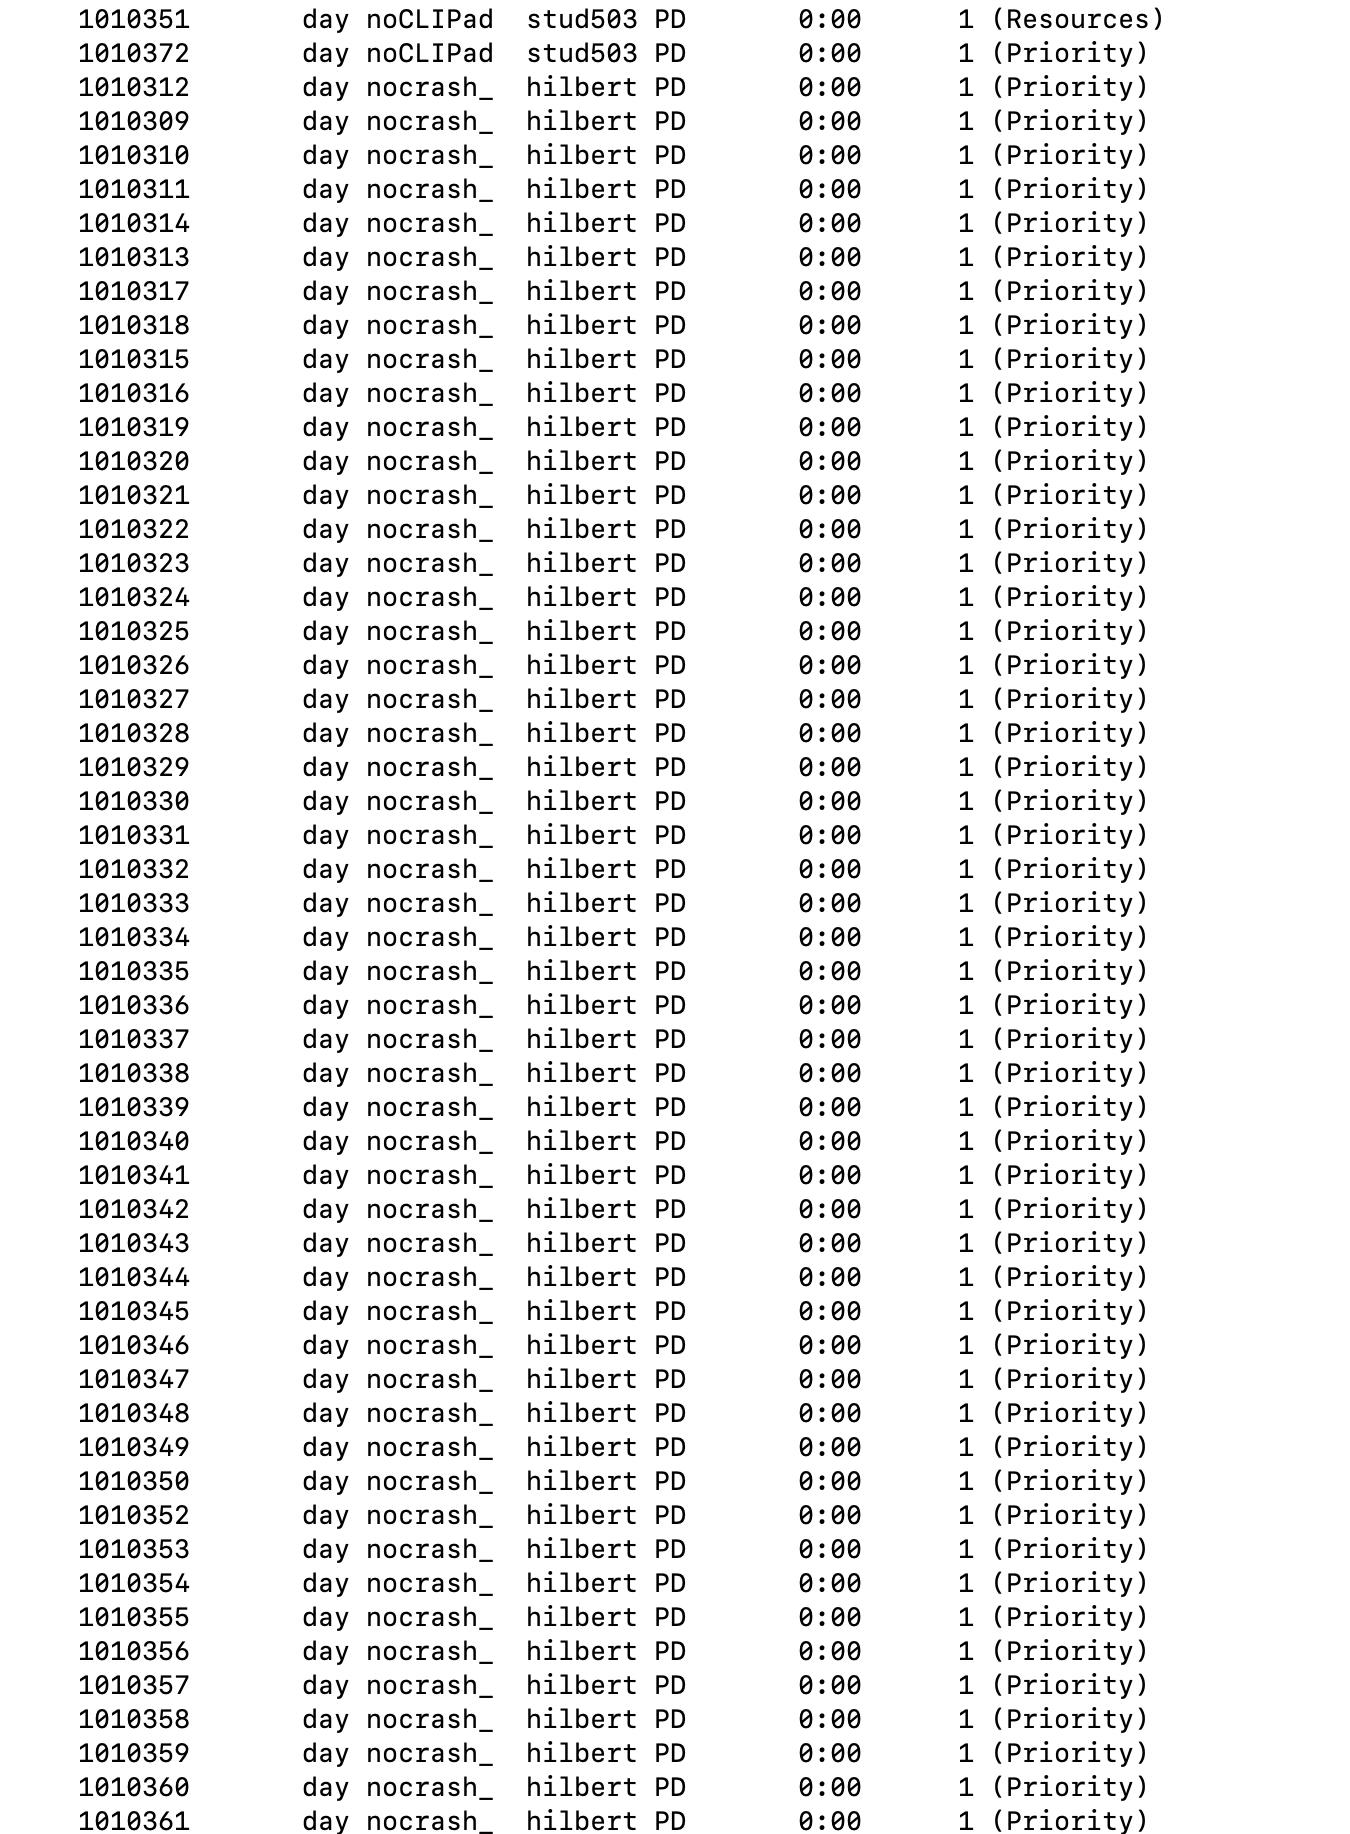
\includegraphics[width=12cm]{figures/hilbertDOS.png}
	\end{center}
\end{frame}

\end{document} 